\documentclass{article}
\usepackage{graphicx}% http://ctan.org/pkg/graphicx
\usepackage{geometry}
 \geometry{
 a4paper,
 left=20mm,
 right=20mm,
 top=20mm,
 bottom=20mm,
 }
 \newcommand{\specialcell}[2][c]{%
  \begin{tabular}[#1]{@{}c@{}}#2\end{tabular}}
\begin{document}
\begin{minipage}{0.45\textwidth}
{\Large Shubham Jain}
\\ 2nd year Undergraduate
\\ Department of Computer Science and Engineering 
\\ Indian Institute of Technology, Kanpur
\\
\\ Email: shubhja@iitk.ac.in
\\  Phone: (+91) 7754916035
\\  Address: Room no. 347, Hall3
\end{minipage}
\begin{minipage}{0.45\textwidth}
\hfill{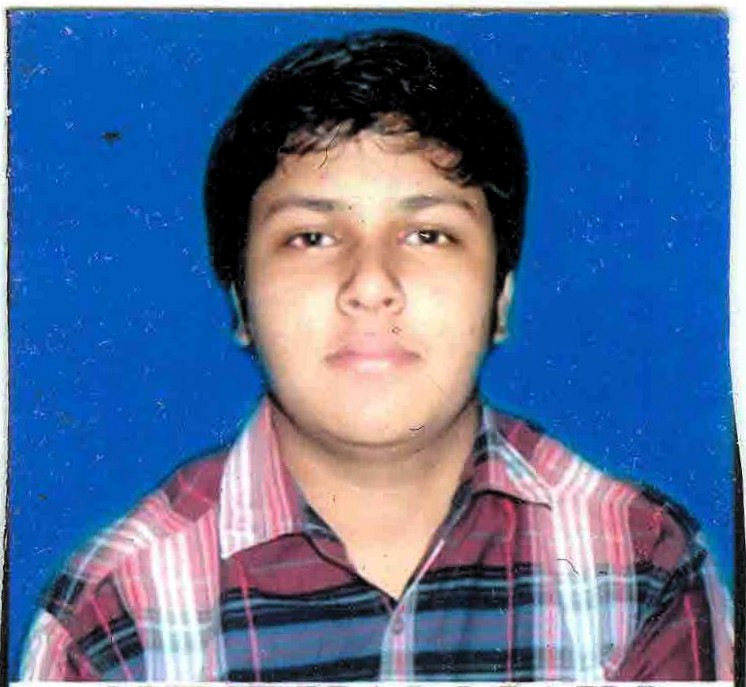
\includegraphics[bb=100 100 700 600,height=3cm,width=3cm]{Photo.jpg}}
\end{minipage}
\\ \vspace{5 mm}
\\
{\large Educational Qualifications}
\\\\
\begin{tabular}{ | c | c | c | c |}\hline
Year & Degree / Certificate & Institute & CPI / \% \\\hline
2017* (Expected) & \specialcell{Bachelor Of Technology,\\Computer Science and Engineering }& \specialcell{Indian Institute Of Technology,\\ Kanpur }& CPI = 10.0/10.0 \\[2.5ex] \hline
2013 & Class XII  (M. P. Board) & Shanti Niketan & 92 \% \\ [1ex] \hline
2011 & Class X (CBSE) & Vatsalya Senior Sec. School & CGPA=9.8/10 \\ [1ex] \hline
\end{tabular}
\\ \\ \\
{\large Achievements}
\begin{description}
 \item[$\bullet $] Secured an All India Rank (AIR) of 210 in IIT-JEE 2013 (JEE ADVANCED) from among 150,000 aspirants
 \item[$\bullet $] Secured an All India Rank (AIR) of 92 in JEE MAINS 2013 from among 1,400,000 aspirants
 \item[$\bullet $] Qualified for ACM ICPC (International Collegiate Programming Contest) Amritapuri Regionals 2013 securing rank 72 among 1500 teams in the Online Round.
 \item[$\bullet $] Secured 60th Rank out of 250 teams in ACM-ICPC Amritapuri Onsite Contest 2014-15 after clearing the Online Round.
\end{description}
\vspace{5 mm}
{\large Transcript}
\\ \\ \vspace{10 mm}
\begin{tabular}{ | c | c | c | c | c |}\hline
Course & Course Type & Title & Units & Grade \\\hline
CHM101A & Compulsory & Chemistry Laboratory & 3 & A\\\hline
ESC101A & Compulsory & Fundamentals of Computing & 14 & A\\\hline
CS201 & Compulsory & Mathematics for Computer Science - I & 9 & A\\\hline
CS210 & Compulsory & Data Structures and Algorithms  & 14 & A\\\hline
PHY103A & Compulsory & Physics -2 & 11 & A \\\hline
MTH101A & Compulsory & Mathematics 1 & 11 & A*\\\hline
\end{tabular}
\end{document}
